The easiest and best studied nonlinear map is the \emph{logistic map} defined as
\begin{equation}
	x_{n+1}=Ax_n(1-x_n)=A(x_n-x_n^2)\quad\text{with}\quad0\leq A\leq4
\end{equation}
\textbf{fixed points} for map is $x_{n+1}=x_n$.
\begin{equation}
	x_n=A(x_n-x_n^2)\quad\rightarrow\quad\tilde{x}_1=0\quad\tilde{x}_2=\frac{A-1}{A}
\end{equation}
As before, we can linearize around these fixed points to determine their stability
\begin{equation*}
	\xi_{n+1}\approx\underbrace{A(1-2\tilde{x})}_{\tilde{A}}\xi_n=\tilde{A}\ \xi_n
\end{equation*}
For the two fixed points $\tilde{x}_1$ and $\tilde{x}_2$ we find
\begin{equation}
	\begin{aligned}
		\tilde{x}_1=0\quad\rightarrow\quad\tilde{A}=A\quad\rightarrow\quad\text{stable for}\ 0\leq A<1\\
		\tilde{x}_2=1-\frac{1}{A}\quad\rightarrow\quad\tilde{A}=A\left\{1-2\left(\frac{A-1}{A}\right)\right\}=2-A\quad\rightarrow\quad\text{stable for}\ 1\leq A\leq3
	\end{aligned}
\end{equation}
These fixed points and their stability can be seen in the bifurcation diagram shown in Figure (\ref{fig:lmbf}).\\
By varying the parameter $A$, the following behavior is observed:
\begin{itemize}
	\item With $A$ between 0 and 1, $x_n\rightarrow0$ as $n\rightarrow\infty$ independent of $x_0$.
	\item With $A$ between 1 and 2, $x_n\rightarrow\dfrac{A-1}{A}$ as $n\rightarrow\infty$ independent of $x_0$.
	\item With $A$ between 2 and 3, $x_n\rightarrow\dfrac{A-1}{A}$ as $n\rightarrow\infty$ but it will fluctuate around that value for some time (converges linearly).
	\begin{figure}[h!]
		\centering
		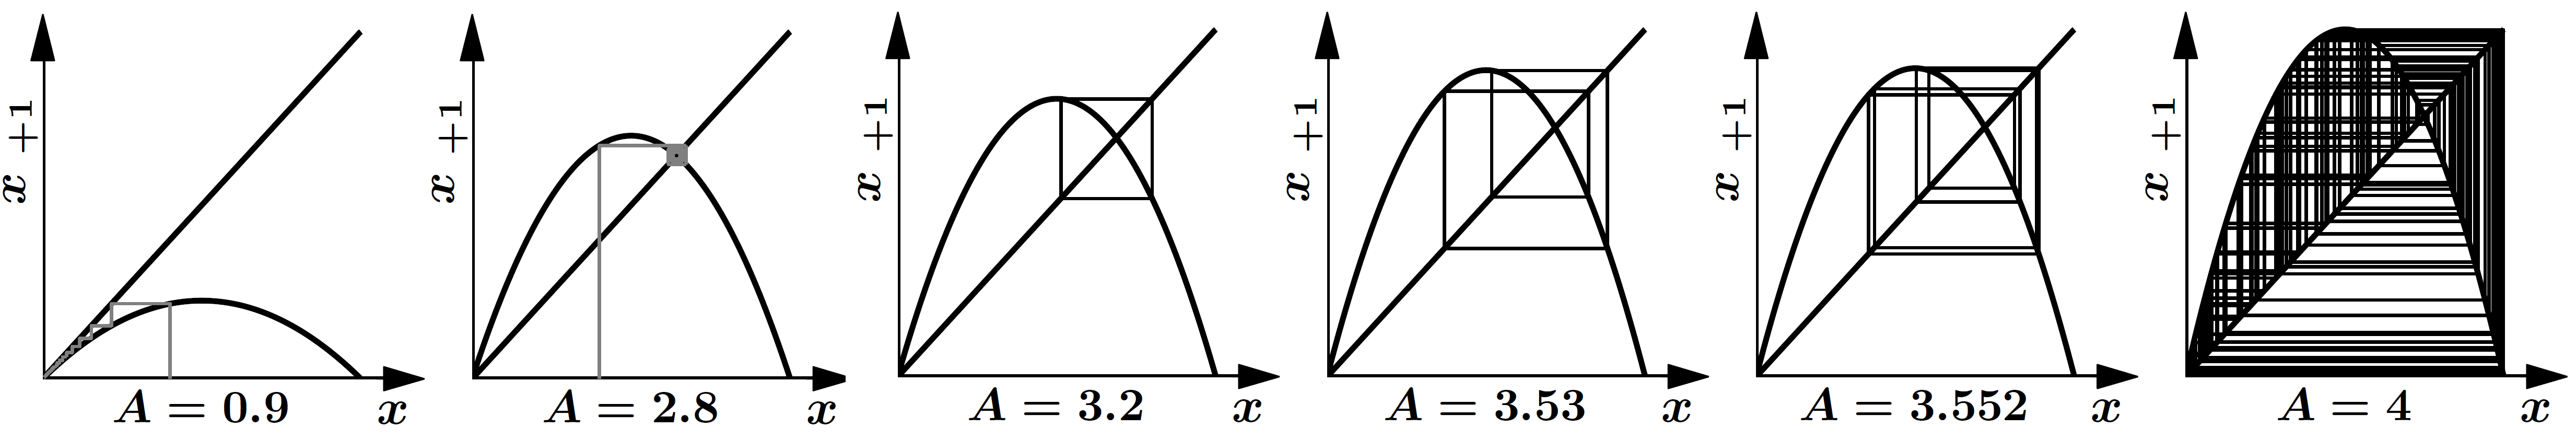
\includegraphics[width=\linewidth]{lm34.png}
		\caption{Stationary states from left to right are fixed points 0 and $\frac{9}{14}$ then orbits with periods of 2, 4 and 8, as well as a chaotic trajectory.}
		\label{fig:lm34}
	\end{figure}
	\item In discrete maps, the analogue to limit cycles in differential equations are periodic orbits of period $m$, where $x_{n+m}=x_n$ is fulfilled.
	Orbits of period 2 are solutions with $x_{n+2}=x_n$
	\begin{equation}
		x_{n+2}=f^{(2)}(x_n)=A^2x_n(1-x_n)(1-Ax_n+Ax_n^2)
	\end{equation}
	The function $f^{(2)}(x_n)$ is called the \emph{second iterate} and has the fixed points
	\begin{equation}
		\tilde{x}_1=0\quad\tilde{x}_2=1-\frac{1}{A}\quad\tilde{x}_{3,4}=\frac{1}{2A}\left\{A+1\pm\sqrt{A^2-2A-3}\right\}
	\end{equation}
	The points $\tilde{x}_1$ and $\tilde{x}_2$ are the fixed points of the map we know already and are unstable for $A>3$.
	It can be shown that the period-2 solution is stable for $3<A<1+\sqrt{6}$.\\
	With $A$ between 3 and $1+\sqrt{6}\approx3.44949$, from almost all $x_0$, $x_n$ will approach permanent oscillations between two values dependent on $A$.
	\item With $A$ between $1+\sqrt{6}$ and 3.54409 (approximately\footnote{This is a root of a $12^{th}$ degree polynomial $4913 + 2108x^2 - 604x^3 - 977x^4 + 8x^5 + 44x^6 + 392x^7 - 193x^8 - 40x^9 + 48x^{10} - 12x^{11} + x^{12}$! So we turn to approximations. :-(}), from almost all $x_0$, $x_n$ will approach permanent oscillations among four values. 
	\item With $A$ increasing beyond 3.54409, from almost all initial conditions $x_0$ will approach oscillations among 8 values.
	This period doubling behavior continues until a period-$\infty$ is reached at a parameter value of $A\approx3.569945672$ and is called \textbf{period-doubling cascade}.
	\item Beyond this point till $A=4$, there is a region of deterministic chaos where the solution is a strange attractor.
	Evidently, this structure in parameter space is a kind of replication of the whole bifurcation diagram on a smaller scale in $x$ and $A$, a feature called \emph{self-similarity}.\\
	This is not the end of the story, however, Figure (\ref{fig:lmbf}) clearly shows regions where the system returns to periodic behavior, even if for only a small range of $\mu$ values.
	These regions are called \textbf{periodic windows}.
	\item The special case of r = 4 can in fact be solved exactly
	\begin{equation}
		x_n=\sin^2(2^n\theta\pi)\quad\text{where}\quad\theta=\frac{1}{\pi}\sini(\sqrt{x_0})
	\end{equation}
	\item Beyond $A=4$, almost all initial values eventually leave the interval $[0,1]$ and diverge.
\end{itemize}
\begin{figure}[h!]
	\centering
	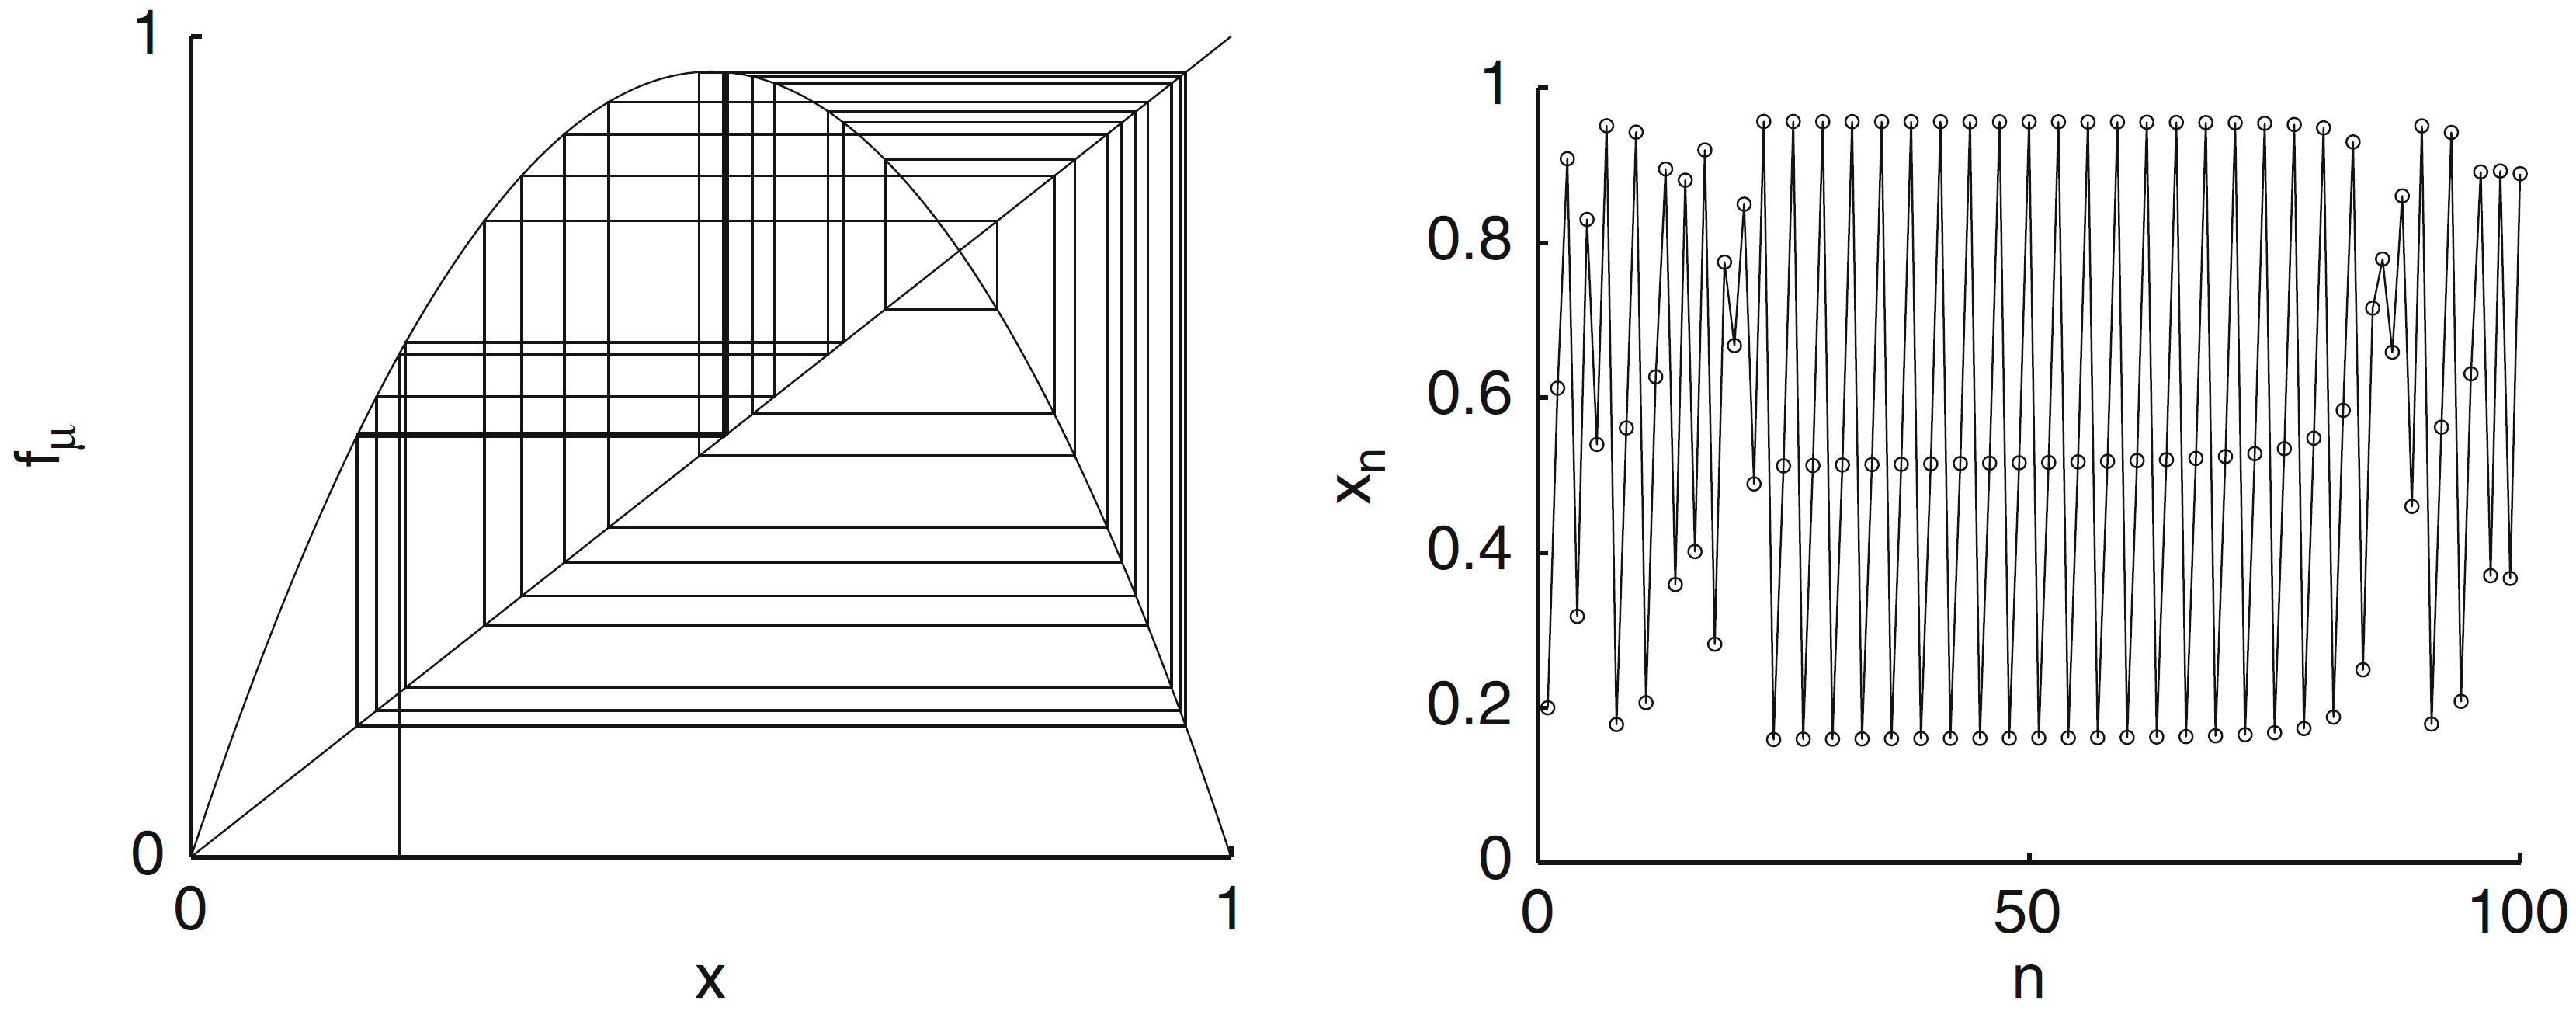
\includegraphics[width=0.5\linewidth]{itmrtc.png}
	\caption{Left: Iterative paths when $\mu=3.8282$ and $x_0=0.2$.\\Right: Time series data.}
	\label{fig:itmrtc}
\end{figure}
\begin{figure}[h!]
	\centering
	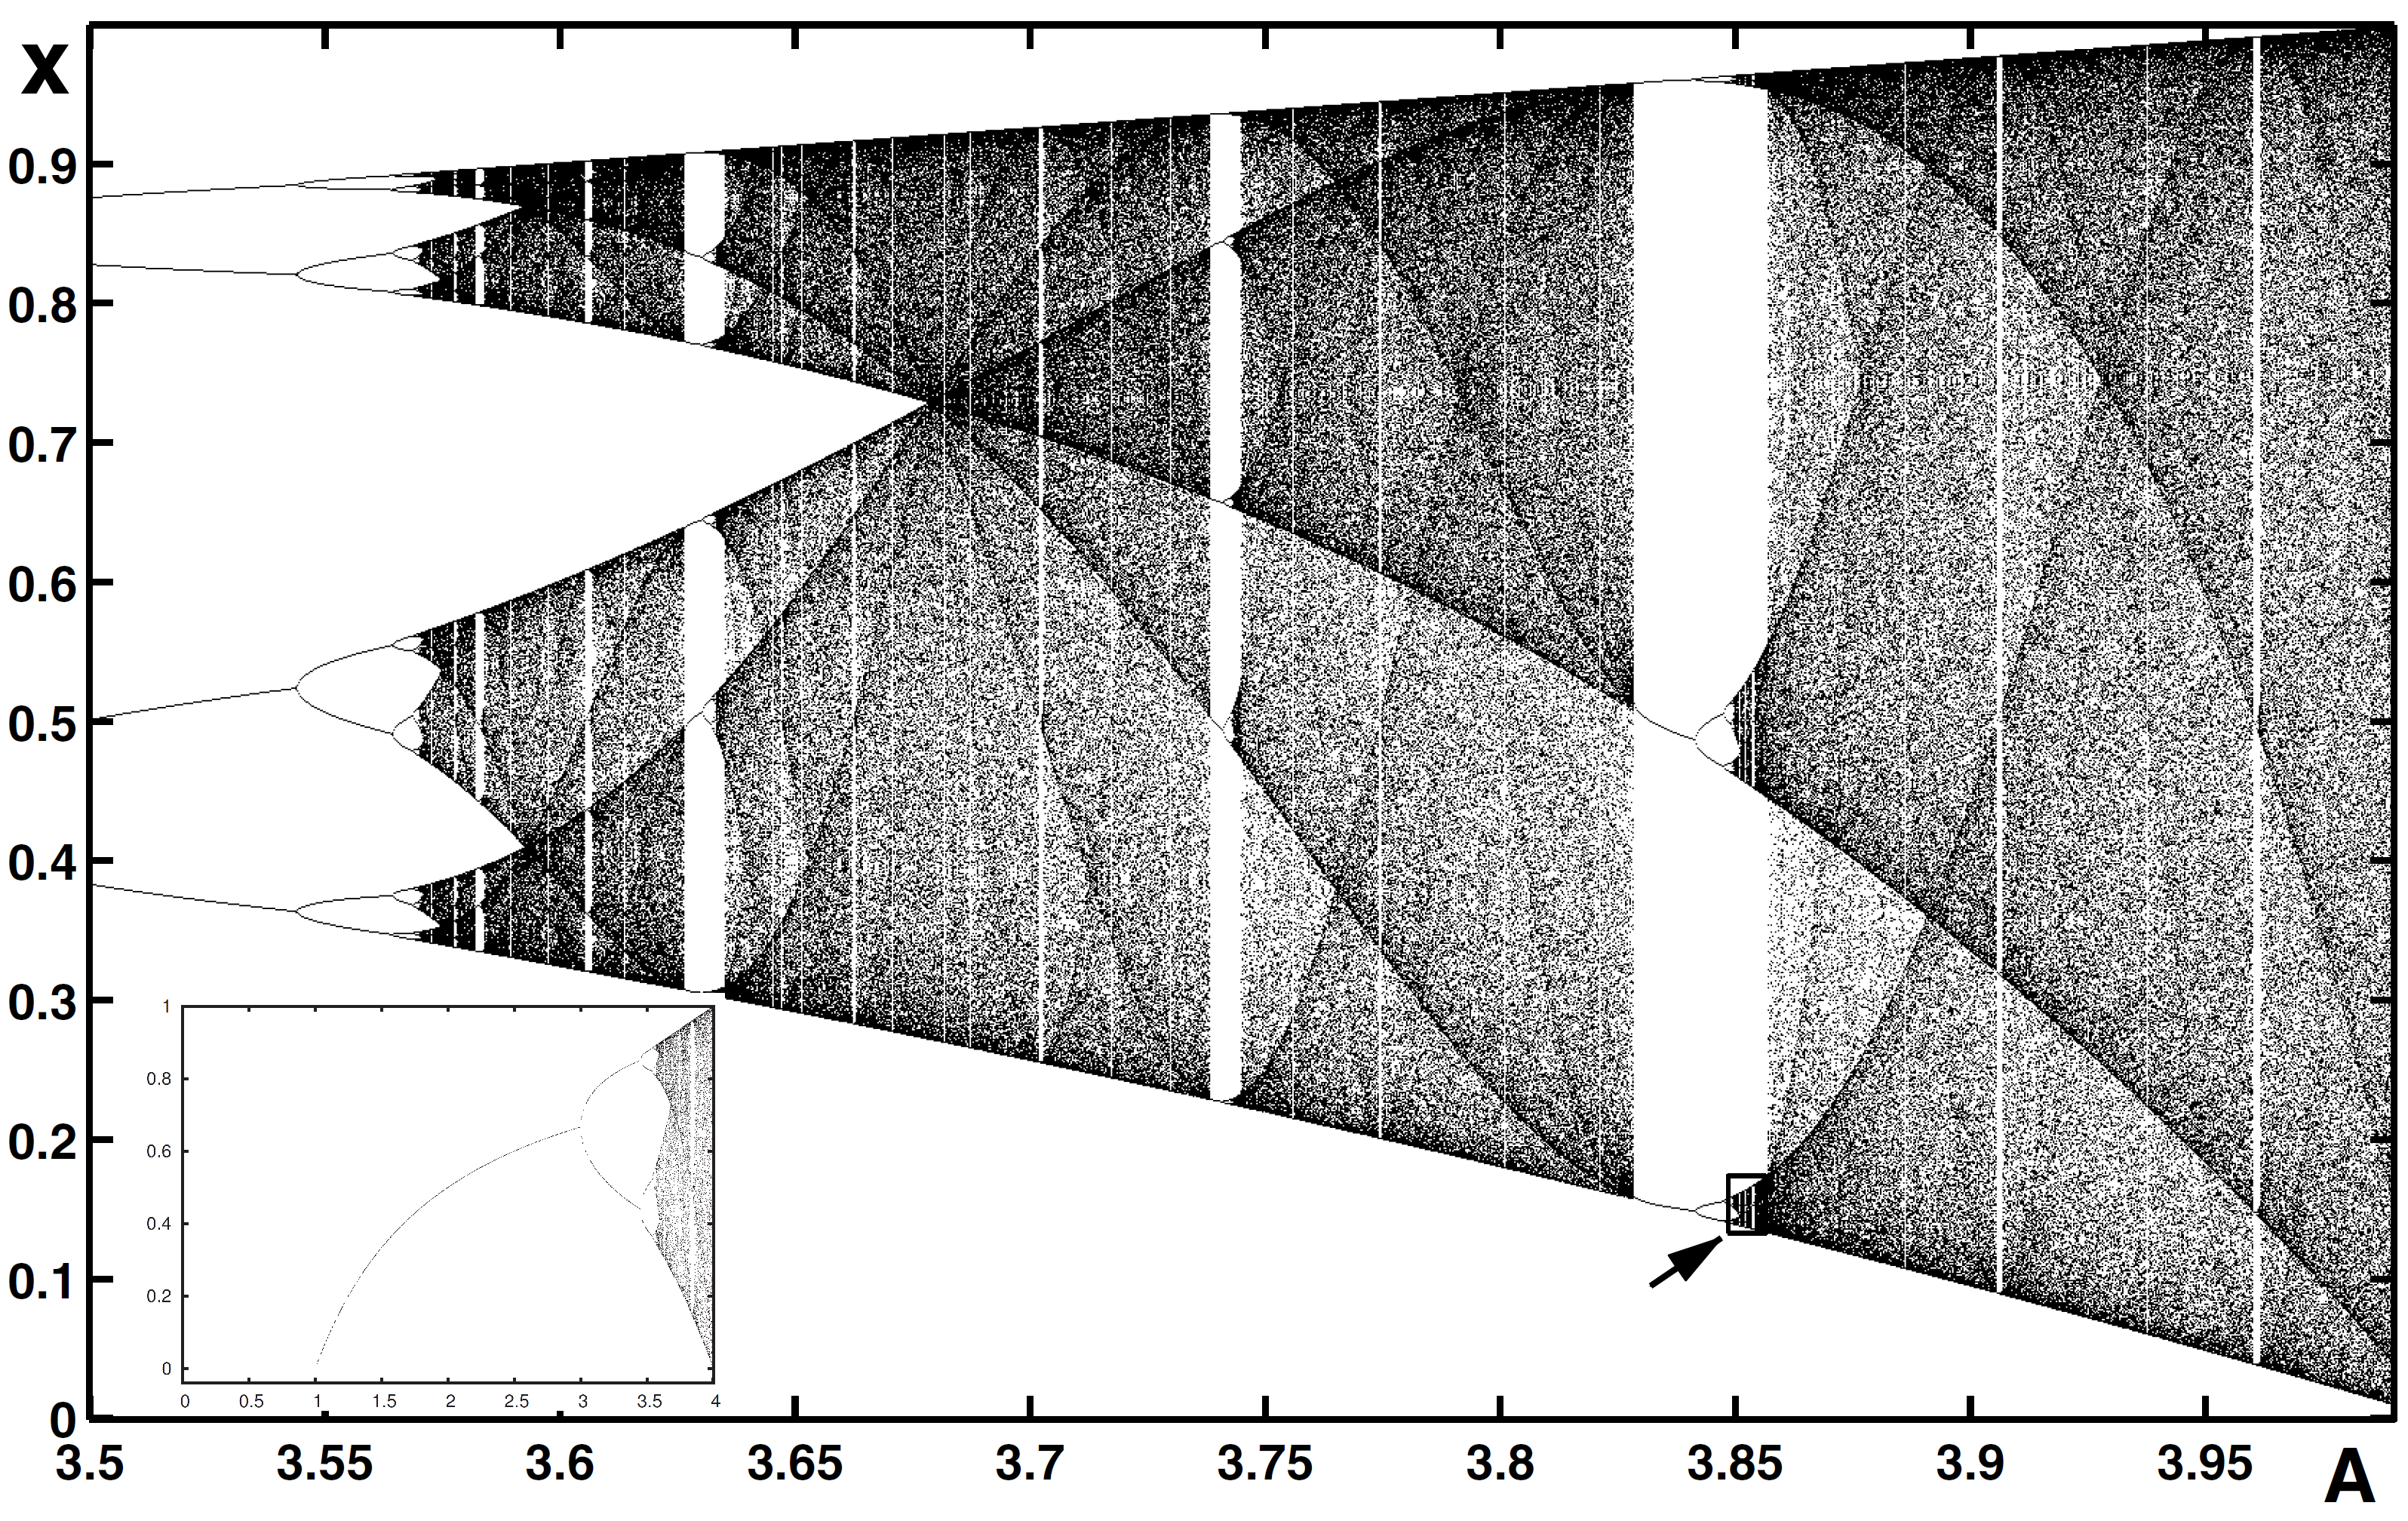
\includegraphics[width=0.7\linewidth]{lmbf.png}
	\caption{Bifurcation diagram for the logistic map for the ‘interesting’ range of the parameter $3.5\leq A\leq4$. The whole parameter range $0\leq A\leq4$ is shown in the insert.}
	\label{fig:lmbf}
\end{figure}
Near to the period-three window, the logistic map can display a new type of behavior known as \textbf{intermittency}, which is almost periodic behavior interrupted by occasional chaotic bursts.
A graphical iteration and time series plot are shown in Figure (\ref{fig:itmrtc}).
As the parameter $\mu$ is increased, the length of the intervals of chaotic bursts become larger and larger until the system becomes fully chaotic.
This phenomenon is known as an \textbf{intermittency route to chaos}.